%\documentclass[onecolumn,amsmath,amssymb]
\documentclass[onecolumn,notitlepage]{revtex4-1}
\renewcommand*\thesection{\arabic{section}}
\usepackage{graphicx}% Include figure files
\usepackage{float} %设置图片浮动位置的宏包
\usepackage{subfigure} %插入多图时用子图显示的宏包
\usepackage{dcolumn}% Align table columns on decimal point
\usepackage{bm}% bold math
\usepackage{amsthm}
\usepackage{amsmath}
\usepackage{amssymb}
\usepackage{color}
\newtheorem{definition}{Definition}%[section]
\newtheorem{algorithm}{Algorithm}%[section]
\newtheorem{theorem}{Theorem}%[section]
\newtheorem{example}{Example}%[section]
\newtheorem{lemma}{Lemma}%[section]
\newtheorem{remark}{Remark}%[section]
\newtheorem{proposition}{Proposition}%[section]
\newtheorem{corollary}{Corollary}%[section]
\newtheorem{conjecture}{Conjecture}%[section]
\newtheorem{result}{Result}%[section]
%\usepackage{ifpdf}

%\renewcommand*\thesection{\arabic{section}}

%%% auxilliary definitions
\def\su{\mathfrak{su}}
\def\u{\mathfrak{u}}
\def\SU{\mathfrak{SU}}
\def\U{\mathfrak{U}}
\definecolor{Red}{rgb}{1,0,0}
\def\vec#1{{\bm #1}}
\def\co#1{{\textcolor{Red}{#1}}}
\def\op#1{#1}
\def\Re{\mathrm{Re}}
\def\ket#1{| #1 \rangle}
\def\bra#1{\langle #1 |}
\def\ip#1#2{\langle #1 | #2 \rangle}
\def\lket#1{| #1 \rangle\!\rangle}
\def\lbra#1{\langle\!\langle #1 |}
\def\lip#1#2{\langle\!\langle #1 \mid #2 \rangle\!\rangle}
\def\comm#1#2{\left\llbracket #1, #2 \right\rrbracket}
\def\ave#1{\langle #1 \rangle}
\def\norm#1{\| #1 \|}
\def\d{\partial}
\def\o{\omega}
\def\RR{\mathbb{R}}
\def\ZZ{\mathbb{Z}}
%% math operators
\def\diag{\operatorname{diag}}
\def\diam{\operatorname{diam}}
\def\pinv{\operatorname{pinv}}
\def\dim{\operatorname{dim}}
\def\supp{\operatorname{supp}}
\def\rank{\operatorname{rank}}
\def\Span{\operatorname{span}}
\def\Sgn{\operatorname{Sgn}}
\def\spec{\operatorname{spec}}
\def\Tr{\operatorname{Tr}}
\def\Ad{\operatorname{Ad}}
%\mathcal symbols
\def\OO{\mathop{\bf O}\nolimits}
\def\Lb{\mathop{\bf L}\nolimits}
\def\Db{\mathop{\bf D}\nolimits}
\def\A{\mathcal{A}}
\def\B{\mathcal{B}}
\def\C{\mathcal{C}}
\def\D{\mathcal{D}}
\def\E{\mathcal{E}}
\def\F{\mathcal{F}}
\def\G{\mathcal{G}}
\def\H{\mathcal{H}}
\def\I{\mathcal{I}}
\def\L{\mathcal{L}}
\def\M{\mathcal{M}}
\def\N{\mathcal{N}}
\def\O{\mathcal{O}}
\def\P{\mathcal{P}}
\def\Q{\mathcal{Q}}
\def\T{\mathcal{T}}
\def\R{\mathbb{R}}
\def\J{\mathcal{J}}
%% blackboard symbols
\def\ONE{\mathbb{I}}
\def\uu{\mathbb{u}}
\def\UU{\mathbb{U}}
\def\GL{\mathbb{GL}}
\def\sp{\mathbb{sp}}
\def\gl{\mathbb{gl}}
\def\so{\mathbb{so}}
\def\o{\omega}
\def\RR{\mathbb{R}}
\def\CC{\mathbb{C}}

%% mathfrak symbols
\def\AA{\mathfrak{A}}
\def\BB{\mathfrak{B}}
\def\DD{\mathfrak{D}}
\def\EE{\mathfrak{E}}
%% other shortcuts
\def\xs{\vec{x}\cdot\vec{\sigma}}
\def\sx{\op{\sigma}_x}
\def\sy{\op{\sigma}_y}
\def\sz{\op{\sigma}_z}
\def\eps{\epsilon}
\def\EEss{\EE_{\rm ss}}
\def\EEinv{\EE_{\rm inv}}
\def\EEcc{\EE_{\rm cc}}
\def\HS{\mathop{\rm HS}}
\def\TR{\mathop{\rm TR}}
\def\ss{\rm ss}

\def\a{\alpha}



\begin{document}

%\title{Indirectly measuring an observable by coupling with a quantum meter}

\title{Quantum Spectral Clustering}

\author{Qingyu Li}

%\date{\today}

\maketitle

\section{Introduction}
Quantum machine learning is an emerging interdisciplinary research area at the intersection of quantum physics and machine learning. The most common use of the term refers to machine learning algorithms for the analysis of classical data executed on a quantum computer.

In recent years, the research in quantum algorithms for machine learning problems has gained substantial momentum. Some of these algorithms include the application of quantum random walk to the community detection in quantum networks, quantum nearest neighbor methods for clustering problems, the deep learning in the context of quantum computing, and an accelerated unsupervised learning algorithm with the help of quantum based subroutines. Furthermore, quantum algorithms for topological and geometric analysis of data and quantum principal component analysis are introduced. The computational complexities of these algorithms are exponentially less than the classical algorithm when the data is accessible on a quantum RAM.

Clustering is one of the most widely used unsupervised machine learning algorithm  for exploratory data analysis, with applications ranging from statistics, computer science, biology to social sciences or psychology. In virtually every scientific field dealing with empirical data, people attempt to get a first impression on their data by trying to identify groups of “similar behavior” in their data. The intuitive goal of clustering is to divide the data points into several groups such that points in the same group are similar and points in different groups are dissimilar to each other. 

Compared to the “traditional algorithms” such as k-means or single linkage, spectral clustering has many fundamental advantages. With roots in graph theory, it uses the spectral properties of the Laplacian matrix to project the data in a low dimensional space where clustering is more efficient. Results obtained by spectral clustering often outperform the traditional approaches, spectral clustering is very simple to implement and can be solved efficiently by standard linear algebra methods.

In this paper, we propose a quantum-enhanced spectral clustering algorithm. We use the phase estimation algorithm and amplitude amplification algorithm to quickly calculate the eigenvalues and eigenvectors of Laplace matrix, and then use the optimized measurement to realize the clustering of logarithmic data points. Before our article, quantum spectral clustering has been studied once. But it has some problems. It doesn't use a mathematical model of spectral clustering but k clustering; it picks the wrong eigenvectors; it just proves that acceleration exists in special cases, not in general.

The remaining part of this paper is organized as follows: in the section II, there is a brief introduction to spectral clustering and K-means algorithm on the classical computers, including the algorithm itself and mathematical knowledge background. Then , in the next section, the quantum spectral clustering will be introduced. Finally, the complexity of the whole process in analyzed and the results are discussed.


\section{the Classical Spectral Clustering}

\subsection{The K-means Clustering}

Spectral clustering algorithms are generally based on obtaining a clustering solution from the eigenvectors of a matrix which represents some form of a given data. It projects a higher-dimensional data vector into a lower-dimensional space where clustering is more efficient. In general, $k$-means algorithm is used to cluster the obtained low-dimensional data vectors. So we first give the description of this algorithm and then describe the spectral clustering.

Given a set of $N$ data vectors, $v_{1},v_{2},\dots,v_{N}$ $k$-means clustering tries to find best $k$ centroids for assumed $k$ number of clusters, $S_{1},…S_{k}$, by minimizing the following objective function:
\begin{align}
    \min(\sum_{c=1}^{k}\sum_{v_{i}\in S_{c}}||v_i-m_c||^2)
\end{align}
Where $m_{c}$ represent the center of the cluster $S_C$. And $||v_i-m_c||^2$ is the Euclidean distance measure between the data point $v_i$ and the center $m_c$. The optimization problem defined by the above obejective function is an NP-hard problem; nonetheless, it can be approximately minimized by using $k$-means algorithm, also known as Lloyd’s algorithm.\\ The steps of this algoritm are as follows:\\
1) Initialize centroids for the clusters;\\
2) Assign each data point to the cluster with the closest centroid.\\
3)Assign the means of data in clusters as the new means: i.e., $m_c=\sum_{v_{i}\in S_c}\frac{v_i}{|S_c|}$\\
4)Repeat step 2 and 3 until there is no change in the means.\\

\subsection{The Spectral Clustering}

In this section, we try to briefly summarize the concept of the spectral clustering. Similarities between data points are most commonly represented by similarity graphs. i.e. undirected weighted graphs in which the vertices $v_i$ and $v_j$ are connected if the data points, $x_i$ and $x_j$ represented by these vertices are similar. And the weights on the edges $w_{ij}$ indicates the amount of the similarity $s_{ij}$ between $x_i$ and $x_j$.

The construction of similarity graph $G(V,E)$ from a given data set ${x_{1},...,x_{N}}$ with pairwise similarities $s_{ij}$ or distance $d_{ij}$ can be done in many different ways. Three of the famous ones are: The undirected $\epsilon$-neighborhood graph; The $k$-nearest neighborhood graph; The fully connected graph.

We usually use the similarity matrix to record the information of the similarity graph. By definition, the similarity matrix $W$ is a adjacency matrix with the matrix elements, $w_{ij}$ representing the weigh on the edge between vertex $v_{i}$ and vertex $v_{j}$. The unnormalized Laplacian
for the graph given by $W$ is defined as:
\begin{align}
    L= W-D,
\end{align}
where $D$ is the digonal degree matrix with diagonal elements $d_{ii} = \sum_{j=1}^N w_{ij}$. The smallest eigenvalues of the laplacian matrix is 0 and the elements of the associated eigenvector are equal to one. The multipliciy $m$ of eigenvalue 0 gives the number of connected components in the graph. Clustering is generally done through the eigenvcetors associated to the first smallest eigenvalues $\lambda_1,...,\lambda_k$ such that $\gamma_{k}=|\lambda_{k}-\lambda_{k+1}|$ gives the largest eigengap among all possible eigengaps.\\
\textbf{Unormalized spectral clustering}\\
\emph{Input}: Similarity matrix $S \in \mathbb{R}^{n\times n}$, number $k$ of clusters to construct.\\
1) Construct a similarity graph by one of the ways described in. Let $W$ be its weighted adjacency matrix.\\
2) Compute the unnormalized Laplacian $L$.\\
3) \textbf{Compute the first $k$ eigenvectors $u_{1},\ldots,u_{k}$ of $L$}.\\
4) Let $U \in \mathbb{R}^{n \times k}$ be the matrix containing the vectors $u_{1},\ldots,u_{k}$ as columns.\\
5) For $i=1,\ldots,n$, let $y_{i} \in \mathbb{R}^{k}$ be the vector corresponding to the $i-$th row of $U$.\\
6) Cluster the points $(y_{i})_{i=1,\ldots,n}$ in $\mathbb{R}^{k}$ with the $k-$means algorithm into clusters $C_{1},\ldots,C_{k}$.\\
\emph{Output}: Clusters $A_{1},\ldots,A_{k}$ with $A_{i}=\{j|y_{j}\in C_{i}\}$



\section{the Quantum Spectral Clustering}

\subsection{The enhanced quantum phase}
In our quantum spectral clustering algorithm, our focus is not on how to construct similarity matrix, which has many different construction methods in the classical algorithm. 
So let's assume that we already have the similarity matrix which is given by $k$-nearest neighbor. 
We can easily construct the Laplacian matrix by the similarity matrix. 
Next, we will process the Laplacian matrix on a quantum computer to analyze its information. 
Similar to the classical spectral clustering algorithm, the quantum spectral clustering algorithm also needs to obtain the eigenvectors corresponding to the first $k$ smallest eigenvalues, and then perform $K$-means clustering on them to obtain the final clustering results. 
Therefore, the quantum spectral clustering algorithm is divided into two steps. 
First, we use the phase estimation algorithm and the amplitude amplification algorithm to find the eigenvectors corresponding the first $k$ smallest eigenvalues of the Laplacian matrix. 
Second, we perform $K$-means clustering on the matrix composed of the eigenvectors to get the final clustering resutls. 
This step is based on the spectral relaxation form of $K$-means clustering.

In order to use the phase estimation to obtain the eigenvectors and eigenvalues of the Laplacian matrix $L$, we first need to consturct the unitary operator $U$ corresponding to $L$. 
$L$ has a good property, it is a $k+1$ sparse matrix and real symmetric matrix. 
So, we can effectively simulation the unitary operator $U=e^{-iLt}$. Suppose $L$ has eigenvalues $\lambda_{j=1,...,N}$ and corresponding eigenvectors $u_{j=1,...,N}$. 
The $U$ has eigenvalues $e^{-i\lambda_{j}t}$ and also corresponding eigenvectors $u_{j=1,...,N}$.

In most articles, people usually use the phase estimation to get the eigenvalues and eigenvectors of the interested matrix. 
The phase estimation needs two registers, the first register is phase register, and the second register is eigenvector regiser. 
In general, people prepare $\frac{1}{\sqrt{N}}\ket{0}\sum_{i=0}^{N-1}\ket{i}$ as the input, and look forward to get $\frac{1}{\sqrt{N}}\sum_{i=0}^{N-1}a_{i}\ket{\lambda_{i}}\ket{u_{i}}$ as the output, where $a_{i}$ is the overlap between eigenstate $\ket{u_{i}}$ and equal superposition state $\frac{1}{\sqrt{N}}\sum_{i=0}^{N-1}\ket{i}$. 
However, if the overlap $a_{i}$ is zero, then the output does not contain $\ket{u_{i}}$'s information. 
For example, the eigenvectors of Pauli $Z$ are $u_{0}=\ket{+}$ and $u_{1}=\ket{-}$. 
If the input state is $\ket{0}\frac{1}{2}(\ket{0}+\ket{1})$, then the output does not contain the $u_{1}$ because of $a_{1}=0$. 
To solve this problem, we put forward an improvement plan. 
We increase the number of registers from 2 to 3, and prepare the second register and the third register to the maximum entangled state. 
So the input is $\ket{0}\frac{1}{\sqrt{N}}\sum_{i=0}^{N-1}\ket{i}\ket{i}$. 
We can prove that 
\begin{align}
    \frac{1}{\sqrt{N}}\sum_{i=0}^{N-1}\ket{i}\ket{i}=\frac{1}{\sqrt{N}}\sum_{i=0}^{N-1}\ket{u_{i}}\ket{u_{i}^{*}},
\end{align}
where $\ket{u_{i}}$ are eigenvectors of $U$ and $\ket{u_{i}^{*}}$ are conjugate of $\ket{u_{i}}$. And the $\frac{1}{\sqrt{N}}\sum_{i=0}^{N-1}\ket{i}\ket{i}$ can be prepared effectively.
The more detial proof is introduced in the appendix.
If the input state is $\ket{0}\frac{1}{N}\sum_{i=0}^{N-1}\ket{i}\ket{i}$, then there will be no $a_{i}=0$ and all of $a_{i}=1$.

We can use the improvement phase estimation which is noted as $U_{pe}$ to get all eigenvalues and eigenvectors of $L$.
\begin{align}
    U_{pe}\ket{0}\frac{1}{\sqrt{N}}\sum_{i=0}^{N-1}\ket{i}\ket{i}=\frac{1}{\sqrt{N}}\sum_{i=0}^{N-1}\ket{\tilde{\lambda_{i}}}\ket{u_{i}}\ket{u_{i}^{*}}.
\end{align}
The error $\epsilon=|\tilde{\lambda_{i}}-\lambda_{i}|^{2}$ depends on the number of qubits in the phase register. Because we don't care what the eigenvalues are, so if the error is small enough, we can ignore it. 

Now we get the all eigenvalues and eigenvectors of $L$. 
The next step is to obtain the eigenvectors corresponding to the first $k$ smallest eigenvalues.
Suppose the first $k$ eigenvalues $\tilde{\lambda_{i=0,...,k-1}} \in Q$, where $Q$ is a range $[0,s]$. 
In the amplitude amplification, we need an 'Black box' which can recognize whether a number is within a certain range. 
In particular, it can know the eigenvalues in $Q$. 
The Oracle can conveniently be represented by a function $f_{O}(x)$. 
By definition, $f_{O}(\lambda)=1$ if $\lambda \in Q$ and $f_{O}(\lambda)=0$ if $\lambda \notin Q$. 
By the Oracle, we can reform
\begin{align}
    \begin{split}
        \frac{1}{\sqrt{N}}\sum_{i=0}^{N-1}\ket{\tilde{\lambda_{i}}}\ket{u_{j}}\ket{u_{j}^{*}} &= \frac{1}{\sqrt{N}}\sum_{\tilde{\lambda_{i}}\in Q}\ket{\tilde{\lambda_{i}}}\ket{u_{j}}\ket{u_{j}^{*}} + \frac{1}{\sqrt{N}}\sum_{\tilde{\lambda_{i}}\notin Q}\ket{\tilde{\lambda_{i}}}\ket{u_{j}}\ket{u_{j}^{*}}\\
        &=\sqrt{\frac{k}{N}}\ket{\alpha}+\sqrt{\frac{N-k}{N}}\ket{\beta}.
    \end{split}
\end{align}
The iteration operator is
\begin{align}
    G=(2\ket{\psi}\bra{\psi}-I)O,
\end{align}
where $\ket{\psi}=\frac{1}{\sqrt{N}}\sum_{i=0}^{N-1}\ket{\tilde{\lambda_{i}}}\ket{u_{i}}\ket{u_{i}^{*}}$.

The effect of $G$ can be understood in a beautiful way by realizing that the oracle operation $O$ performs a reflection about the state $\ket{\beta}$ in the plan defined by $\ket{\alpha}$ and $\ket{\beta}$.
That is, $O(a\ket{\alpha}+b\ket{\beta})=(-a\ket{\alpha}+b\ket{\beta})$.
Similarly, $2\ket{\psi}\bra{\psi}-I$ also performs a reflection in the plane defined by $\ket{\alpha}$ and $\ket{\beta}$, about the state $\ket{\psi}$. And the product of two reflcetion is a rotaion. The $R=O(\sqrt{N/k})$ iterations must be performed in order to obtain a superposition state of the firs $k$ eigenvalues and corresponding eigenvectors with high probability. After enough iterations, the output state may not be exactly what we want. But the error can be ignored. By the iterations, suppose we get the
\begin{align}
    \ket{\phi}=\frac{1}{\sqrt{k}}\sum_{\tilde{\lambda_{i}}\in Q}\ket{\tilde{\lambda_{i}}}\ket{u_{i}}\ket{u_{i}^{*}}.
\end{align}
Since we don't need information about the eigenvalues, we need to untangle the state. So we apply the $U_{pe}^{\dagger}$ to the state $\ket{\phi}$. Then we obtain
\begin{align}
    U_{pe}^{\dagger}\ket{\phi}=\ket{0}\frac{1}{\sqrt{k}}\sum_{\tilde{\lambda_{i}}\in Q}\ket{u_{i}}\ket{u_{i}^{*}}.
\end{align}
We note $\frac{1}{\sqrt{k}}\sum_{\tilde{\lambda_{i}}\in Q}\ket{u_{i}}\ket{u_{i}^{*}}$ as $\ket{\phi'}$. We just want to obtain the first register in $\ket{\phi'}$, so we need to apply the partial trace to $\ket{\phi'}\bra{\phi'}$ to extract information of the first register.
\begin{align}
    \rho_{1}=Tr_{2}\bigg[\frac{1}{k}\sum_{\tilde{\lambda_{i}}\in Q}\ket{u_{i}}\ket{u_{i}^{*}}\sum_{\tilde{\lambda_{j}}\in Q}\bra{u_{j}}\bra{u_{j}^{*}} \bigg]=\frac{1}{k}\sum_{\tilde{\lambda_{i}}\in Q}\ket{u_{i}}\bra{u_{i}}.
\end{align}
The first $k$ eigenvectors of $L$ are noted as $A=[u_{1},...,u_{k}]$. We can find $AA^{T}=\sum_{i=1}^{k}\ket{u_{j}}\bra{u_{j}}$, it is precisely the state we got form the above operation.

\begin{figure}[H] %H为当前位置,!htb为忽略美学标准,htbp为浮动图形
    \centering %图片居中
    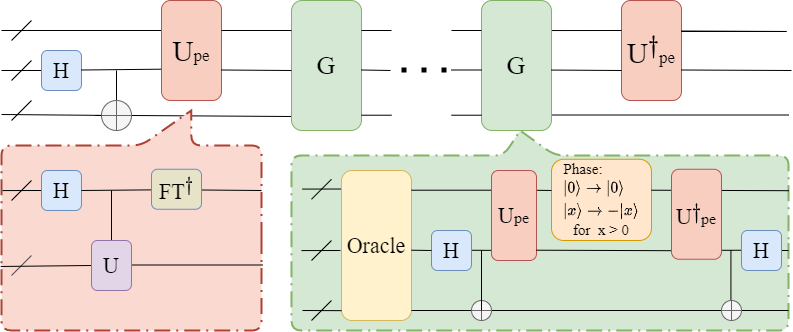
\includegraphics[width=0.7\textwidth]{image//circuit.png} %插入图片,[]中设置图片大小,{}中是图片文件名
    \caption{The quantum circuit of quantum spectral clustering,$U=e^{2\pi iL}$, the \em{Oracle} can recognize the first $k$ eigenvalues} %最终文档中希望显示的图片标题
    \label{Fig.main2} %用于文内引用的标签
\end{figure}

\subsection{Optimized measurement algorithm}
Now, let's move on to second step. In classical $K$-means clustering sepctral relaxation is usually used to transform $K$-means clustering to the trace maximization problem. Given a set of $M$-dimensional data vectors $b_{i=1,..,N}$, the $M$-by-$N$ data matrix $B$ is composed of $[b_{1},...,b_{N}]$. Find the best partition of B can be reformed to find the optimal $N$-by-$K$ indicator matrix $X$ which satisfies
\begin{align}
    \max_{X^TX=I_{k}} trace(X^TB^TBX),\label{8}
\end{align}
where $K$ is the number of cluster. We can rewrite equation(\ref{8}) as 
\begin{align}
    \max_{X^TX=I_{k}} trace(B^TBXX^T),
\end{align}
where $XX^T$ is a $N$-by-$N$ hermitian matrix. In the process of spectral clustering, we need apply $K$-means to the column vector of $A=[u_{1},...,u_{k}]$. So let $B=A^T$, the second step is find the indicator matrix $X$ which satisfies
\begin{align}
    \begin{split}
        \max_{X^TX=I_{k}} trace(\frac{1}{k}AA^TXX^T)&=\max_{X^TX=I_{k}} trace(\frac{1}{k}\sum_{i=1}^{k}\ket{u_{i}}\bra{u_{i}} XX^T)\\
        &=\max_{X^TX=I_{k}} trace(\rho_{1} XX^T)
    \end{split}
\end{align} 
If we can construct the observable $M=XX^T$ and the density operator $\rho = \frac{1}{k}\sum_{i=1}^{j}\ket{u_{i}}\bra{u_{i}}$. The problem is transformed to find the maximum value of expectation of measurements. We can optimize the structure of observables $M$ to achive the maximum value. The upper bound of max trace is the sum of the largest $k$ eigenvalues of $\rho_{1}$. We can know, $\rho_{1}$'s eigenvalues are $(n-k)$ 0 eigenvalues and $k$ $\frac{1}{k}$ eigenvalues. So the maximum value of trace is $k\frac{1}{k}=1$.

Classically, if we want to get the final clustering result, we need to fully know the eigenmatrix $A$ or the covariance matrix $AA^T$, and then do $k$-means clustering for it. However, in quantum, if we want to know the eigenmatrix, we need to do quantum tomography on the quantum system. This is terrible. The cost of quantum tomography is expensive. So, what can we do to get the clustering information. We propose a feasible scheme to obtain the result of clustering by measurement. We have no prior knowledge of what kind of measurement operator will get the optimal result. Therefore, we need a set of methods to update the measurement operator and multiple measurements to ensure that we get an optimal solution. We use the local search algorithm to guide the measurement process. 
The objective function is 
\begin{align}
    \max_{X^TX=I_{k}} trace(\rho_{1} XX^T).
\end{align}
Our optimization strategy can be divided into the following steps.
1.Construct an initial indicator matrix $X$. and get $m=trace(\rho_{1} XX^T)$.\\
2.Randomly select a row of $X$, swap the elements ,then get $X$'s neighborhood $X'$. i.e.[0,1] is replaced [1,0].\\
3.if $m'=trace(\rho_{1} X'X^{'T}) \geq m$, then update the $X=X'$. Repeat 2.\\
4.if $m'\leq m$. Repeat 2.

When we repaet the measurement enough times, the finally result $X$ is approximation of the optimal solution $X*$. However, if we want to get the optimal solution, the cost is very high. In practice, we often do not take the optimal algorithm to get the optimal solution. Through the above algorithm, we can successfully extract the clustering information. it's complexity is lower than that of quantum tomography.

\begin{figure}[H] %H为当前位置,!htb为忽略美学标准,htbp为浮动图形
    \centering %图片居中
    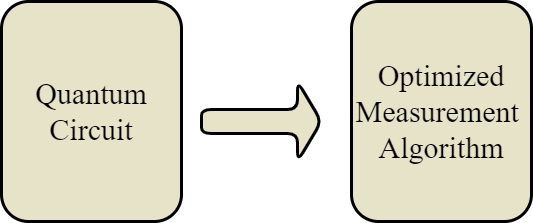
\includegraphics[width=0.7\textwidth]{image//algorithm.png} %插入图片,[]中设置图片大小,{}中是图片文件名
    \caption{The whole process of the quantum spectral clustering} %最终文档中希望显示的图片标题
    \label{Fig.main2} %用于文内引用的标签
\end{figure}


\section{numerical simulation}
In order to verify that our algorithm is feasible, we present numerical simulations on simple synthetic datasets made of two concentric circles, as in the original work on spectral clustering, in order to benchmark the quality of the quantum algorithm. 
These simulation are made with a classical computer that simulates the quantum spectral clustering. Because of the performance limitations of classical computers, we cannot simulate higher-dimensional situations. In our simulation, the phase register has six qubits, the eigenstate register has four qubits, and the other four qubits are used to entangle with the eigenstate register. So the whole quantum system has 14 qubits and the number of points is $2^4=16$.
\begin{figure}[H]
    \centering 
    \subfigure[initial graph]{
    \label{Fig.sub.1}
    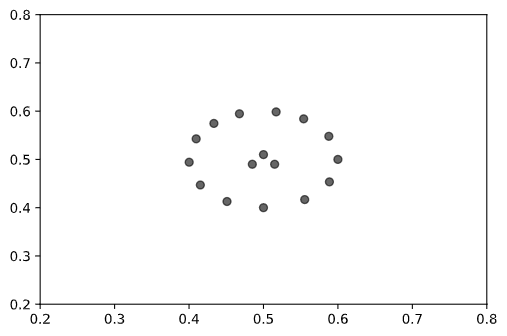
\includegraphics[width=0.3\textwidth]{image//allblack.png}}
    \subfigure[quantum spectral cluster]{
    \label{Fig.sub.2}
    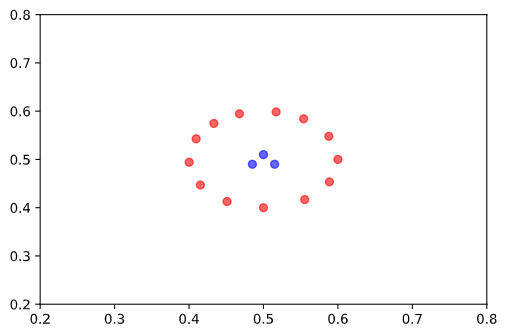
\includegraphics[width=0.3\textwidth]{image//spectral.png}}
    \subfigure[k-means cluster]{
    \label{Fig.sub.3}
    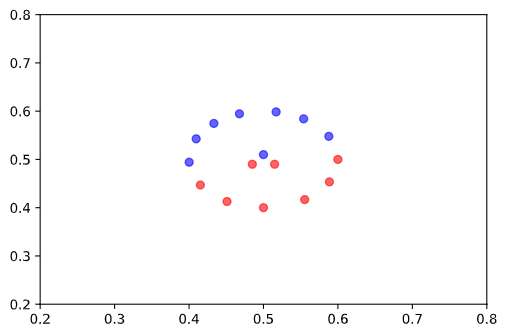
\includegraphics[width=0.3\textwidth]{image//kmeans.png}}
    \caption{quantum sepctral cluster}
    \label{Fig.main}
\end{figure}

\begin{figure}[H]
    \centering 
    \subfigure[initial graph]{
    \label{Fig.sub.1}
    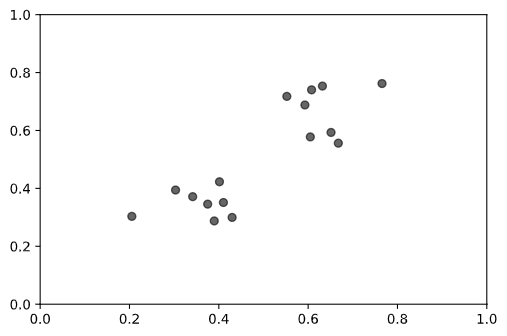
\includegraphics[width=0.3\textwidth]{image//scat.png}}
    \subfigure[quantum spectral cluster]{
    \label{Fig.sub.2}
    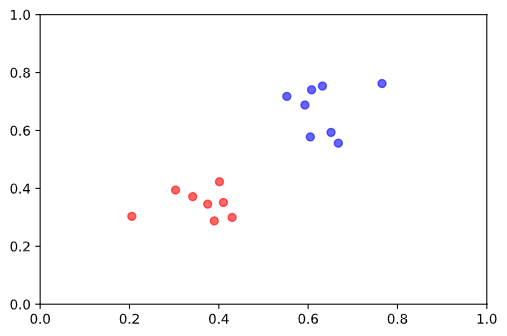
\includegraphics[width=0.3\textwidth]{image//scat1.png}}
    \caption{quantum sepctral cluster}
    \label{Fig.main}
\end{figure}

\section{Appendix}

\subsection{The maximum entangle state}

Suppose we have a unitary operator $U$, if we want to get the eigenvalues and eigenvectors of $U$. We can use the phase estimation algorithm to do this. We prepare $\ket{0}\frac{1}{\sqrt{N}}\sum_{i=0}^{N-1}\ket{i}$ as the input state and construct the $control$-$U$. The output state is $\frac{1}{\sqrt{N}}\sum_{i=0}^{N-1}a_{i}\ket{\lambda_{i}}\ket{u_{i}}$, where $\lambda_{i}$ and $\ket{u_{i}}$ are eigenvalues and eigenvectors of U respectively and $a_{i}$ is the overlap between the equal superposition state and $\ket{u_{i}}$.
However, there is a potential problem with this. If some $a_{i}=0$, means the overlap between $\ket{u_{i}}$ and equal superposition state is zero, the output does not contain the information of $\ket{u_{i}}$.

We conclude that if we input the maximum entangled state, we will avoid this problem. The maximum entangle state $\sum_{j}\ket{j}\ket{j}$ consists of two register. We declare that the $\sum_{j}|j\rangle|j\rangle = \sum_{j}\ket{u_{j}}\ket{u_{j}^{*}}$, where $\ket{u_{j}}$ is the eigenvcetors of $U$. Suppose $U$ is a normal matrix. And we can represent $u_{j}$ as $\sum_{i=0}^{N-1}a_{i,j}\ket{i}$.

Now we give a detial proof of the argument above. First of all, let's prove a lemma. From the knowledge of matrix theory, we know the $\sum_{j}\ket{u_{j}}\bra{u_{j}} = I$. And we suppose $\ket{m}$ as a arbitrary orthonormal basis.
Thus, we can get 
\begin{align}
    \begin{split}
        \ket{m}  &= \sum_{j}\ket{u_{j}}\bra{u_{j}}\ket{m}       \\
        &=\sum_{j}\bigg[\sum_{i}a_{ij}\ket{i}\sum_{k}a_{kj}^*\bra{k}\bigg]\ket{m}  \\
        &= \sum_{j}\sum_{i}\sum_{k} a_{ij} a_{kj}^*\ket{i}\ip{k}{m}  \\
        &= \sum_{j}\sum_{i}a_{ij} a_{mj}^*\ket{i}.
    \end{split}
\end{align}

Then we can proof the final conclusion.
\begin{align}
    \begin{split}
        \sum_{j}\ket{u_{j}}|u_{j}^*\rangle &= \sum_{j}\bigg[ \sum_{k}a_{kj}|k\rangle \sum_{i}a_{ij}^*\ket{i}\bigg]\\
        &=  \sum_{i}\bigg[\sum_{j}\sum_{k}a_{kj}a_{ij}^*|k\rangle\bigg]\ket{i}\\
        &= \sum_{i}\ket{i}\ket{i}
    \end{split}
\end{align}


\end{document}
